\documentclass[aspectratio=169, 12pt]{beamer}

% --- Theme ---
\usetheme{Madrid}
\usecolortheme{seahorse}
\setbeamertemplate{navigation symbols}{}
\setbeamertemplate{footline}[frame number]
\setbeamercolor{frametitle}{bg=structure.fg!15, fg=structure.fg}
\setbeamercolor{block title}{bg=structure.fg!20, fg=structure.fg!90!black}
\setbeamercolor{block body}{bg=structure.fg!5}
\setbeamercolor{block title alerted}{bg=red!20, fg=red!80!black}
\setbeamercolor{block body alerted}{bg=red!5}
\setbeamercolor{block title example}{bg=green!20, fg=green!50!black}
\setbeamercolor{block body example}{bg=green!5}

\usepackage[utf8]{inputenc}
\usepackage[T1]{fontenc}
\usepackage[french]{babel}
\usepackage{graphicx}
\usepackage{booktabs}
\usepackage{multicol}
\usepackage{tikz}

\title[FacePredictor]{FacePredictor}
\subtitle{Prediction d'age, de genre et d'ethnicite par Deep Learning}
\author{Ako Christian \and Calrd Similien \and Noe Cervera \and Dhanoush Kessavane}
\institute{IUT de Villetaneuse --- Universite Sorbonne Paris Nord}
\date{SAE BUT3 Informatique --- 2025--2026}

\begin{document}

% ============================================================
% SLIDE 1 --- Page de titre
% ============================================================
\begin{frame}
\titlepage
\vspace{-1cm}
\centering
\small Encadrement : Bilal Faye \& Hanane Azzag --- LIPN, CNRS UMR 7030
\end{frame}

% ============================================================
% SLIDE 2 --- Sommaire
% ============================================================
\begin{frame}{Sommaire}
\tableofcontents
\end{frame}

% ============================================================
\section{Objectif du projet}
% ============================================================
\begin{frame}{Objectif du projet}

\begin{block}{Mission}
Developper une application Android capable de predire \textbf{l'age}, le \textbf{genre} et \textbf{l'ethnicite} d'une personne a partir d'une photo de son visage grace au Deep Learning.
\end{block}

\vspace{0.5cm}

\begin{columns}[T]
\begin{column}{0.48\textwidth}
\textbf{Cote Machine Learning}
\begin{itemize}
    \item TensorFlow / Keras
    \item TensorFlow Lite
    \item Dataset UTKFace (23\,708 images)
    \item Scikit-learn (metriques)
\end{itemize}
\end{column}
\begin{column}{0.48\textwidth}
\textbf{Cote Android}
\begin{itemize}
    \item Kotlin + Android SDK 34
    \item MediaPipe (detection visage)
    \item Firebase Auth + Firestore
    \item CameraX (temps reel)
\end{itemize}
\end{column}
\end{columns}

\end{frame}

% ============================================================
\section{Dataset UTKFace}
% ============================================================
\begin{frame}{Dataset UTKFace}

\begin{columns}[T]
\begin{column}{0.55\textwidth}
\begin{block}{Description}
\begin{itemize}
    \item \textbf{23\,708 images} de visages recadres
    \item 3 labels : age (0--116), genre (H/F), ethnicite (5 classes)
    \item Split stratifie : 70\% train / 15\% val / 15\% test
\end{itemize}
\end{block}
\end{column}

\begin{column}{0.42\textwidth}
\begin{alertblock}{Desequilibre}
\begin{itemize}
    \item White : $\sim$45\%
    \item Black : $\sim$20\%
    \item Asian / Indian : $\sim$15\% chacun
    \item Other : $\sim$5\%
\end{itemize}
$\rightarrow$ Focal Loss + poids de classe
\end{alertblock}
\end{column}
\end{columns}

\vspace{0.4cm}

\begin{exampleblock}{Preprocessing}
Resize 224$\times$224 --- Data augmentation (flip, crop, luminosite, contraste) --- Mixed precision float16
\end{exampleblock}

\end{frame}

% ============================================================
\section{Strategie 1 : Trois modeles specialises}
% ============================================================
\begin{frame}{Strategie 1 --- Trois modeles specialises}

\begin{block}{Architecture par modele}
Backbone \textbf{EfficientNetB0} (ImageNet) $\rightarrow$ GlobalAvgPool $\rightarrow$ BatchNorm $\rightarrow$ Dropout $\rightarrow$ Dense
\end{block}

\vspace{0.3cm}

\begin{columns}[T]
\begin{column}{0.32\textwidth}
\centering
\textbf{Age}\\[0.2cm]
Dense(1), lineaire\\
Huber Loss ($\delta$=5)\\[0.2cm]
\textit{MAE $\approx$ 6.2 ans}
\end{column}

\begin{column}{0.32\textwidth}
\centering
\textbf{Genre}\\[0.2cm]
Dense(1), sigmoid\\
BCE (smoothing 0.05)\\[0.2cm]
\textit{Accuracy $\approx$ 90\%}
\end{column}

\begin{column}{0.32\textwidth}
\centering
\textbf{Ethnicite}\\[0.2cm]
Dense(5), softmax\\
Focal Loss ($\gamma$=2)\\[0.2cm]
\textit{Accuracy $\approx$ 70\%}
\end{column}
\end{columns}

\vspace{0.4cm}

\begin{exampleblock}{Entrainement en 2 phases}
Phase 1 : backbone gele (15 epochs, lr=1e-3) --- Phase 2 : fine-tune 15 couches (40 epochs, lr=1e-5, batch=4)
\end{exampleblock}

\end{frame}

% ============================================================
\section{Strategie 2 : Modele multi-tache MoE}
% ============================================================
\begin{frame}{Strategie 2 --- Mixture of Experts (MoE)}

\begin{columns}[T]
\begin{column}{0.55\textwidth}
\begin{block}{Architecture}
\begin{itemize}
    \item Backbone \textbf{EfficientNetB0} partage
    \item 3 tetes MoE independantes
    \item Chaque tete : \textbf{4 experts} (MLP) + 1 \textbf{gating network}
    \item Le gating network route chaque image vers l'expert le plus adapte
\end{itemize}
\end{block}

\begin{exampleblock}{Poids des pertes}
Age = 0.3 --- Genre = 1.5 --- Ethnicite = 2.0
\end{exampleblock}
\end{column}

\begin{column}{0.42\textwidth}
\begin{block}{Entrainement 3 phases}
\begin{enumerate}
    \item \textbf{Warmup} (25 ep.) --- backbone gele
    \item \textbf{Fine-tune partiel} (20 ep.) --- 15 couches
    \item \textbf{Fine-tune etendu} (15 ep.) --- 30 couches
\end{enumerate}
\end{block}

\vspace{0.2cm}
\small
\textit{Nettoyage memoire GPU entre chaque phase (RTX 4050, 6 Go VRAM)}
\end{column}
\end{columns}

\end{frame}

% ============================================================
\section{Strategie 3 : Comparaison des backbones}
% ============================================================
\begin{frame}{Strategie 3 --- Comparaison des backbones}

\begin{table}
\centering
\small
\begin{tabular}{lcccccc}
\toprule
\textbf{Backbone} & \textbf{Genre Acc} & \textbf{Genre AUC} & \textbf{Eth Acc} & \textbf{Age MAE} & \textbf{Temps} & \textbf{Score} \\
\midrule
\textbf{EfficientNetB0} & \textbf{90.1\%} & \textbf{96.4\%} & \textbf{68.3\%} & 6.19 & 15 min & \textbf{9.17} \\
ResNet50 & 89.9\% & 96.5\% & 66.9\% & 5.87 & 33 min & 9.15 \\
MobileNetV3Large & 88.5\% & 95.3\% & 67.8\% & 7.11 & 11 min & 9.02 \\
MobileNetV2 & 85.0\% & 93.2\% & 55.7\% & 7.59 & 13 min & 8.37 \\
\bottomrule
\end{tabular}
\end{table}

\vspace{0.3cm}

\begin{block}{Conclusion}
\textbf{EfficientNetB0} selectionne : meilleur compromis precision / taille / vitesse.
ResNet50 quasi egal mais \textbf{5$\times$ plus gros} (30M vs 5M parametres) et 2$\times$ plus lent.
\end{block}

\end{frame}

% ============================================================
\section{Interpretabilite (Grad-CAM)}
% ============================================================
\begin{frame}{Interpretabilite --- Grad-CAM}

\begin{block}{Qu'est-ce que Grad-CAM ?}
Genere des \textbf{cartes de chaleur} montrant les zones de l'image que le modele considere decisives pour chaque prediction.
\end{block}

\vspace{0.3cm}

\begin{columns}[T]
\begin{column}{0.32\textwidth}
\begin{exampleblock}{Age}
\begin{itemize}
    \item Rides, texture de peau
    \item Cheveux gris
    \item Rondeur du visage
\end{itemize}
\end{exampleblock}
\end{column}

\begin{column}{0.32\textwidth}
\begin{exampleblock}{Genre}
\begin{itemize}
    \item Forme de la machoire
    \item Pilosite faciale
    \item Structure osseuse
\end{itemize}
\end{exampleblock}
\end{column}

\begin{column}{0.32\textwidth}
\begin{exampleblock}{Ethnicite}
\begin{itemize}
    \item Teint de la peau
    \item Forme des yeux/nez
    \item Proportions du visage
\end{itemize}
\end{exampleblock}
\end{column}
\end{columns}

\vspace{0.3cm}
\centering
\small\textit{Le modele analyse uniquement les pixels --- pas d'infrarouge ni de capteur special.}

% AJOUTER ICI : 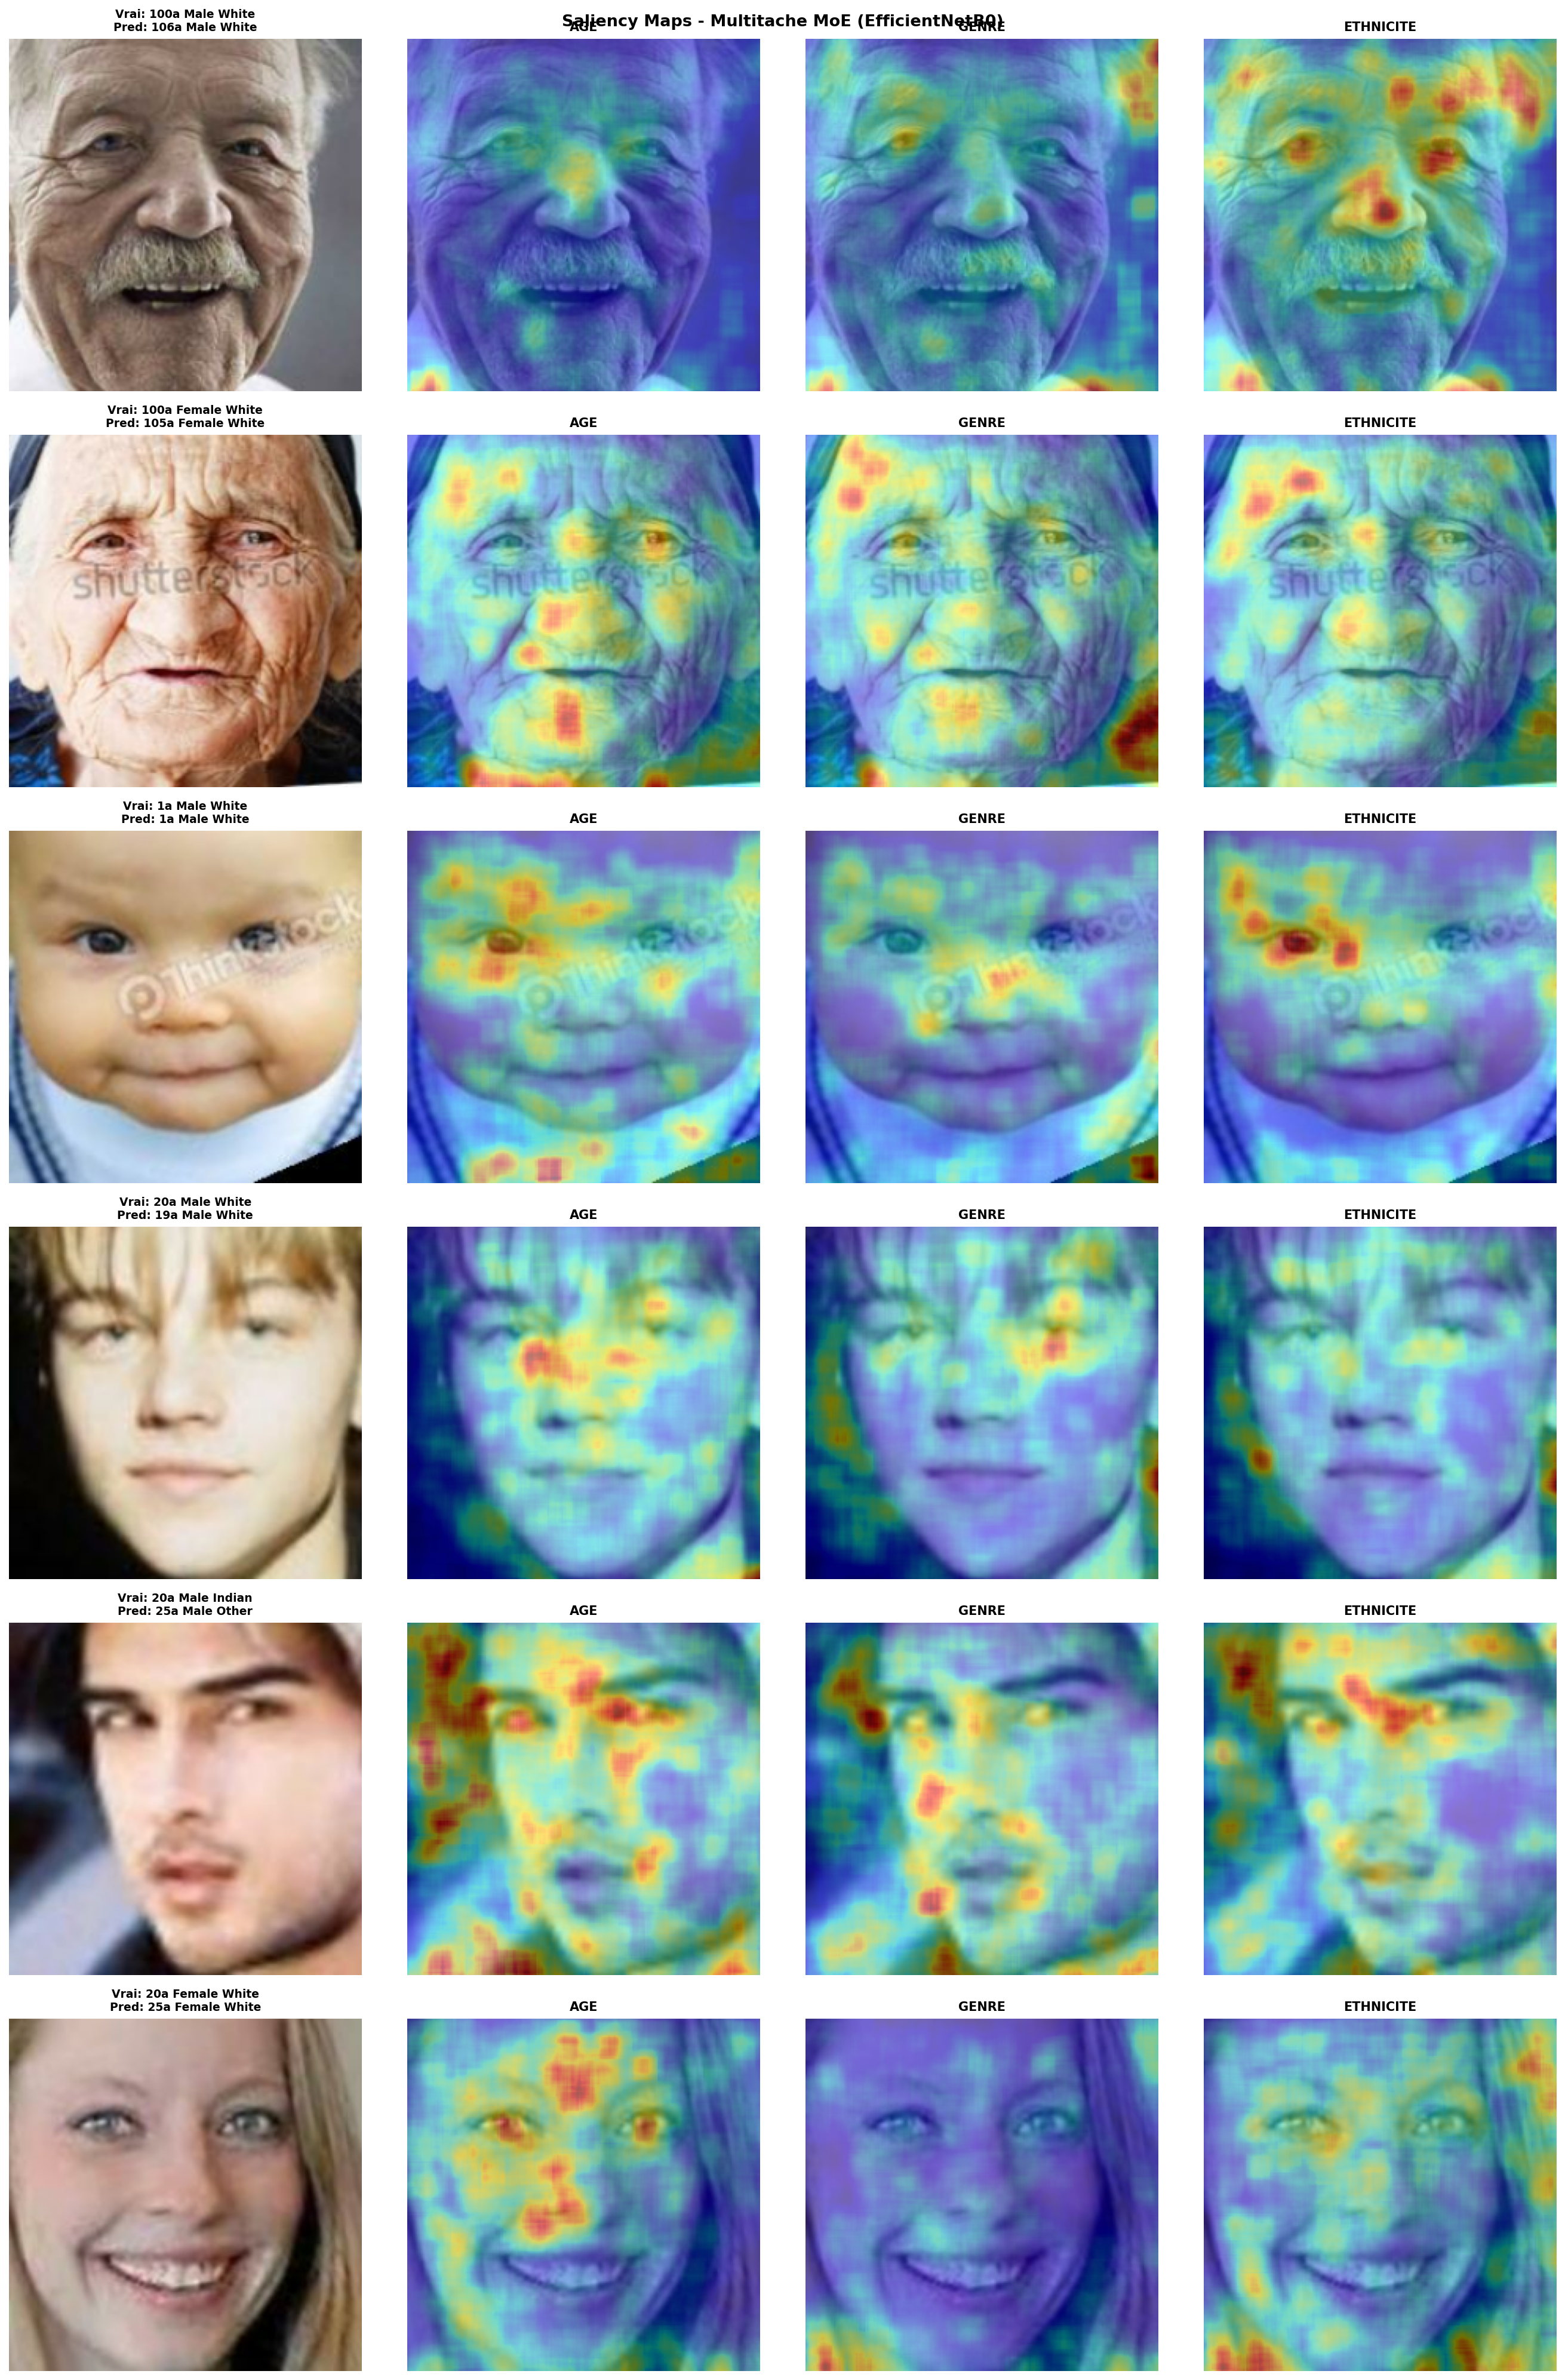
\includegraphics[width=\textwidth]{training/output_v2/gradcam_multitache.png}

\end{frame}

% ============================================================
\section{Application Android}
% ============================================================
\begin{frame}{Application Android --- Fonctionnalites}

\begin{columns}[T]
\begin{column}{0.48\textwidth}
\begin{block}{Prediction}
\begin{itemize}
    \item \textbf{4 modes} : MoE Expert (defaut), Oriente V2, Multitache, Hybride
    \item Camera frontale / arriere
    \item Import galerie
    \item \textbf{Temps reel} (bonus)
    \item Detection visage MediaPipe
\end{itemize}
\end{block}
\end{column}

\begin{column}{0.48\textwidth}
\begin{block}{Compte \& UX}
\begin{itemize}
    \item Auth Firebase (Email + Google)
    \item Historique avec filtres
    \item Profil : stats, securite, export JSON
    \item \textbf{Mode sombre} complet
    \item Tutoriel premiere connexion
    \item Design Material 3 ``Tech bleu/gris''
\end{itemize}
\end{block}
\end{column}
\end{columns}

\vspace{0.3cm}

\begin{alertblock}{Modele par defaut}
\textbf{MoE Expert} avec backbone EfficientNetB0, entraine lors de ce projet (17 Mo en TFLite).
\end{alertblock}

% AJOUTER ICI : screenshots de l'app

\end{frame}

% ============================================================
\section{Resultats finaux}
% ============================================================
\begin{frame}{Resultats finaux --- Modele MoE (defaut)}

\begin{table}
\centering
\begin{tabular}{llc}
\toprule
\textbf{Tache} & \textbf{Metrique} & \textbf{Resultat} \\
\midrule
\textbf{Genre} & Accuracy & \textbf{90.7\%} \\
 & AUC & 96.4\% \\
 & AP / ARI / NMI & 95.3\% / 0.663 / 0.554 \\
\midrule
\textbf{Ethnicite} & Accuracy & \textbf{70.8\%} \\
 & AUC & 90.6\% \\
 & AP / ARI / NMI & 80.8\% / 0.452 / 0.408 \\
\midrule
\textbf{Age} & MAE & \textbf{6.36 ans} \\
 & MSE & 86.3 \\
 & R$^2$ & 0.778 \\
\bottomrule
\end{tabular}
\end{table}

\vspace{0.2cm}
\centering
\small Toutes les metriques du sujet calculees : Accuracy, AUC, AP, MAE, MSE, R$^2$, ARI, NMI

% AJOUTER ICI : 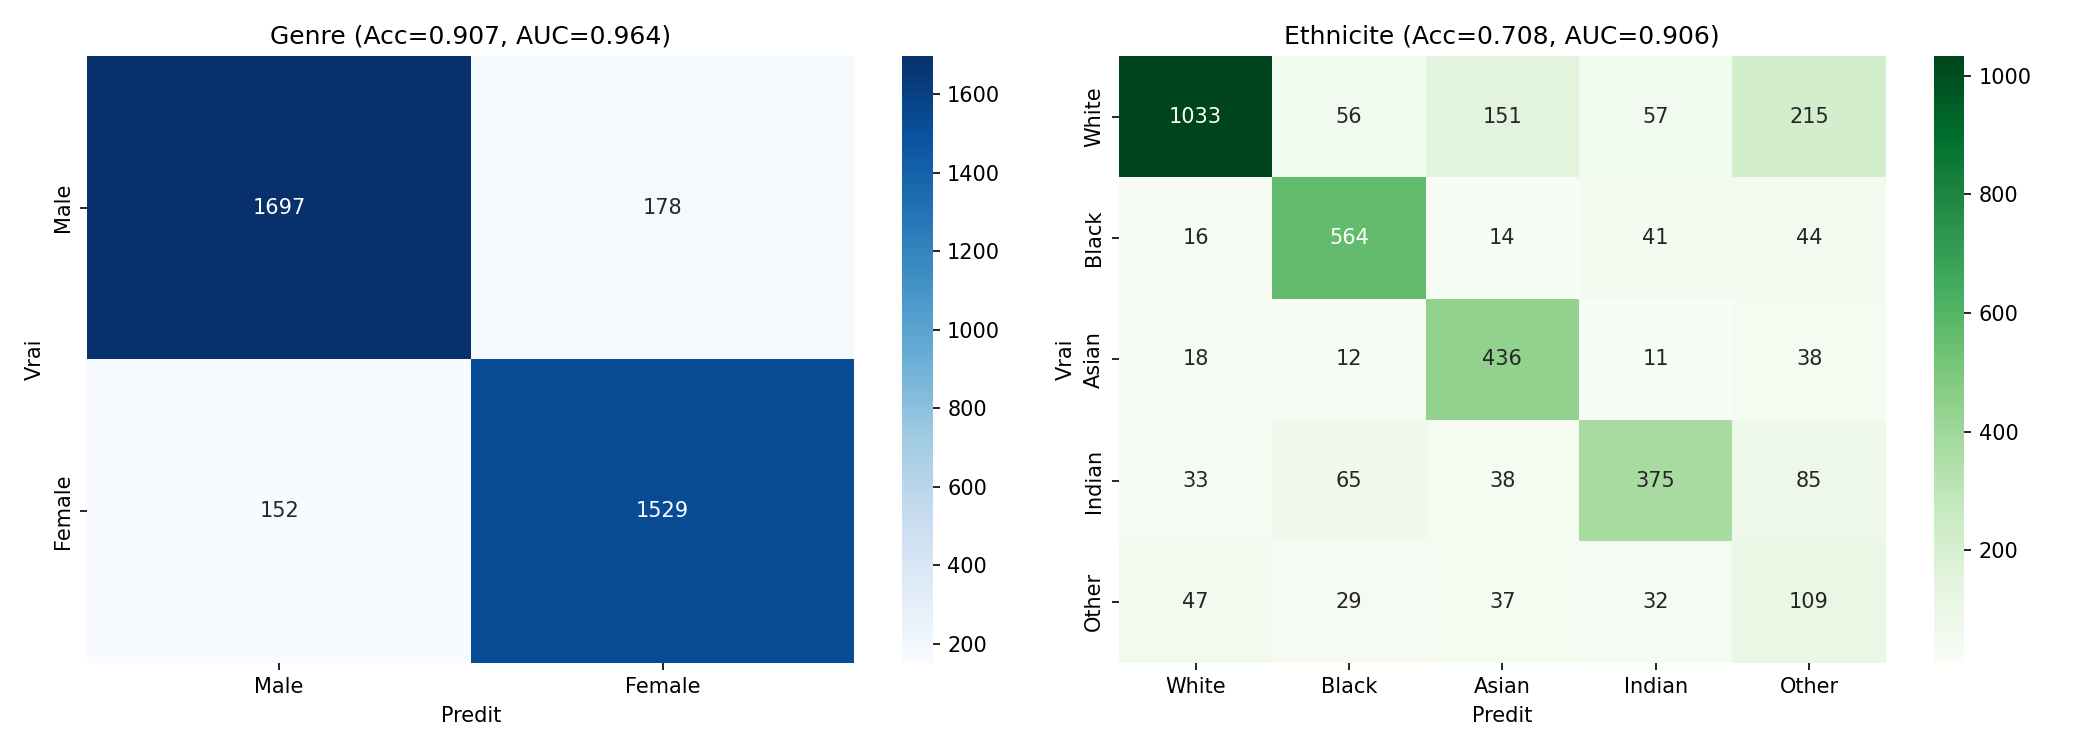
\includegraphics{training/output_v2/multitask_confusion_matrices.png}

\end{frame}

% ============================================================
\section{Difficultes et solutions}
% ============================================================
\begin{frame}{Difficultes rencontrees \& solutions}

\begin{columns}[T]
\begin{column}{0.48\textwidth}

\begin{alertblock}{VRAM limitee (6 Go)}
Batch size reduit a 4, 15 couches max debloquees, VRAM plafonnee a 5 Go, nettoyage memoire entre phases.
\end{alertblock}

\vspace{0.2cm}

\begin{alertblock}{Dataset desequilibre}
Focal Loss + poids de classe inversement proportionnels. Accuracy ``Other'' reste $\sim$50\%.
\end{alertblock}

\end{column}

\begin{column}{0.48\textwidth}

\begin{alertblock}{Confusion Asian / Indian}
Traits visuels proches --- limite inherente au dataset. $\sim$15\% de confusion croisee.
\end{alertblock}

\vspace{0.2cm}

\begin{alertblock}{Reproductibilite}
Seeds fixes (numpy, tensorflow, random) pour des resultats deterministes entre executions.
\end{alertblock}

\end{column}
\end{columns}

\end{frame}

% ============================================================
\section{Conclusion}
% ============================================================
\begin{frame}{Conclusion et perspectives}

\begin{block}{Bilan}
\begin{itemize}
    \item Les \textbf{3 strategies} de modelisation implementees avec succes
    \item Application Android \textbf{fonctionnelle et professionnelle}
    \item Performances solides : 90.7\% genre, 70.8\% ethnicite, 6.36 MAE age
    \item Fonctionnalites avancees : temps reel, mode sombre, export, Grad-CAM
\end{itemize}
\end{block}

\vspace{0.3cm}

\begin{exampleblock}{Perspectives}
\begin{itemize}
    \item Dataset plus grand et mieux equilibre
    \item Architectures plus recentes (EfficientNetV2, Vision Transformers)
    \item Quantification int8 pour deploiement plus leger
    \item Detection multi-visages
\end{itemize}
\end{exampleblock}

\end{frame}

% ============================================================
% SLIDE FIN
% ============================================================
\begin{frame}
\centering
\vspace{1cm}
{\Huge\textbf{Merci pour votre attention}}

\vspace{1cm}
{\Large Questions ?}

\vspace{1cm}
\small
Ako Christian --- Calrd Similien --- Noe Cervera --- Dhanoush Kessavane\\[0.3cm]
IUT de Villetaneuse --- Universite Sorbonne Paris Nord --- 2025--2026\\[0.3cm]
\texttt{github.com/optmlako2004/face-analysis-deep-learning}
\end{frame}

\end{document}